\section{BPTT (backpropagation through time)}
通時的誤差逆伝播法
## モデルの定義
ライブラリの読み込み.
\lstinputlisting[language=julia]{./text/solve-credit-assignment-problem/bptt/003.jl}
\lstinputlisting[language=julia]{./text/solve-credit-assignment-problem/bptt/004.jl}
\lstinputlisting[language=julia]{./text/solve-credit-assignment-problem/bptt/005.jl}
\jl{w_in}は入力層から再帰層への重み,\jl{w_rec}は再帰重み,\jl{w_out}は出力重みである.
\lstinputlisting[language=julia]{./text/solve-credit-assignment-problem/bptt/007.jl}
## 7.9.2 更新関数の定義
\lstinputlisting[language=julia]{./text/solve-credit-assignment-problem/bptt/009.jl}
\subsection{正弦波の学習}
例として正弦波を出力するRNNを考える.入力1,中間64, 出力2のRNNである.
\lstinputlisting[language=julia]{./text/solve-credit-assignment-problem/bptt/011.jl}
入力と訓練データの確認をする.
\lstinputlisting[language=julia]{./text/solve-credit-assignment-problem/bptt/013.jl}
\begin{figure}[ht]
	\centering
	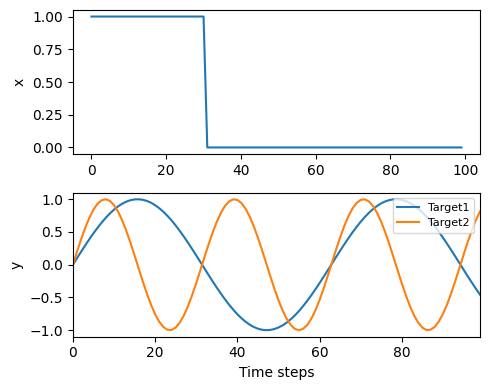
\includegraphics[scale=0.8, max width=\linewidth]{./fig/solve-credit-assignment-problem/bptt/cell013.png}
	\caption{cell013.png}
	\label{cell013.png}
\end{figure}
モデルの定義をする.
\lstinputlisting[language=julia]{./text/solve-credit-assignment-problem/bptt/015.jl}
学習を実行する.
\lstinputlisting[language=julia]{./text/solve-credit-assignment-problem/bptt/017.jl}
損失の推移を確認する.
\lstinputlisting[language=julia]{./text/solve-credit-assignment-problem/bptt/019.jl}
\begin{figure}[ht]
	\centering
	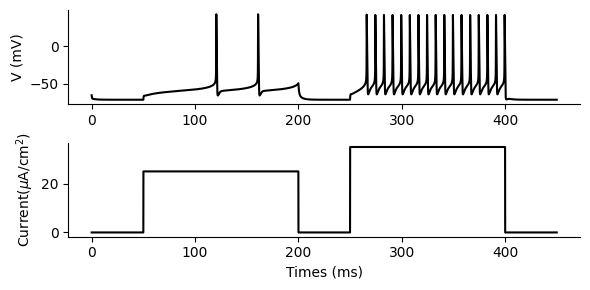
\includegraphics[scale=0.8, max width=\linewidth]{./fig/neuron-model/hodgkin-huxley/cell019.png}
	\caption{cell019.png}
	\label{cell019.png}
\end{figure}
## 学習後の出力の確認
\lstinputlisting[language=julia]{./text/solve-credit-assignment-problem/bptt/021.jl}
見やすいように出力のピークに応じて中間層のユニットをソートする.
\lstinputlisting[language=julia]{./text/solve-credit-assignment-problem/bptt/023.jl}
出力層,中間層の出力を描画する.
\lstinputlisting[language=julia]{./text/solve-credit-assignment-problem/bptt/025.jl}
\begin{figure}[ht]
	\centering
	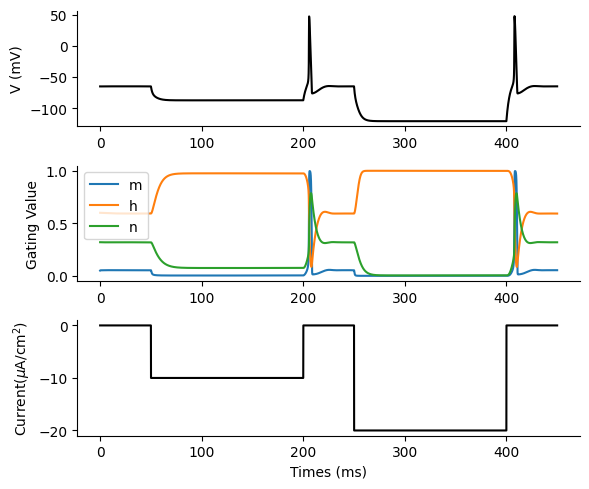
\includegraphics[scale=0.8, max width=\linewidth]{./fig/neuron-model/hodgkin-huxley/cell025.png}
	\caption{cell025.png}
	\label{cell025.png}
\end{figure}
